%% I need this here to get rid of the stupid "preprint submitted" shit on the front matter.
\documentclass[preprint,12pt]{elsarticle}
\makeatletter
\def\ps@pprintTitle{%
 \let\@oddhead\@empty
 \let\@evenhead\@empty
 \def\@oddfoot{}%
 \let\@evenfoot\@oddfoot}

%% Use the option review to obtain double line spacing
%% \documentclass[preprint,review,12pt]{elsarticle}

%% Use the options 1p,twocolumn; 3p; 3p,twocolumn; 5p; or 5p,twocolumn
%% for a journal layout:
%% \documentclass[final,1p,times]{elsarticle}
%% \documentclass[final,1p,times,twocolumn]{elsarticle}
%% \documentclass[final,3p,times]{elsarticle}
%% \documentclass[final,3p,times,twocolumn]{elsarticle}
%% \documentclass[final,5p,times]{elsarticle}
%% \documentclass[final,5p,times,twocolumn]{elsarticle}


%% The graphicx package provides the includegraphics command.
\usepackage{graphicx}
\usepackage{caption}
\usepackage{subcaption}
%% The amssymb package provides various useful mathematical symbols
\usepackage{amssymb}
%% The amsthm package provides extended theorem environments
%% \usepackage{amsthm}
\usepackage{qtree}
%% The lineno packages adds line numbers. Start line numbering with
%% \begin{linenumbers}, end it with \end{linenumbers}. Or switch it on
%% for the whole article with \linenumbers after \end{frontmatter}.
\usepackage{lineno}

\usepackage{color}
\usepackage{listings}
\definecolor{dkgreen}{rgb}{0,0.6,0}
\definecolor{gray}{rgb}{0.5,0.5,0.5}
\definecolor{mauve}{rgb}{0.58,0,0.82}
\definecolor{backcolour}{rgb}{1,0.95,0.84}


\lstset{
  language=R,
  backgroundcolor=\color{backcolour}, 
  aboveskip=3mm,
  belowskip=3mm,
  showstringspaces=false,
  columns=flexible,
  basicstyle={\small\ttfamily},
  numbers=none,
  numberstyle=\tiny\color{gray},
  keywordstyle=\color{blue},
  commentstyle=\color{dkgreen},
  stringstyle=\color{mauve},
  breaklines=true,
  breakatwhitespace=true,
  tabsize=3
}


%% natbib.sty is loaded by default. However, natbib options can be
%% provided with \biboptions{...} command. Following options are
%% valid:

%%   round  -  round parentheses are used (default)
%%   square -  square brackets are used   [option]
%%   curly  -  curly braces are used      {option}
%%   angle  -  angle brackets are used    <option>
%%   semicolon  -  multiple citations separated by semi-colon
%%   colon  - same as semicolon, an earlier confusion
%%   comma  -  separated by comma
%%   numbers-  selects numerical citations
%%   super  -  numerical citations as superscripts
%%   sort   -  sorts multiple citations according to order in ref. list
%%   sort&compress   -  like sort, but also compresses numerical citations
%%   compress - compresses without sorting
%%
%% \biboptions{comma,round}

% \biboptions{}

\journal{Mike}

\begin{document}

\begin{frontmatter}

%% Title, authors and addresses

\title{Predicting Baseball Hall Of Fame Inductions}

%% use the tnoteref command within \title for footnotes;
%% use the tnotetext command for the associated footnote;
%% use the fnref command within \author or \address for footnotes;
%% use the fntext command for the associated footnote;
%% use the corref command within \author for corresponding author footnotes;
%% use the cortext command for the associated footnote;
%% use the ead command for the email address,
%% and the form \ead[url] for the home page:
%%
%% \title{Title\tnoteref{label1}}
%% \tnotetext[label1]{}
%% \author{Name\corref{cor1}\fnref{label2}}
%% \ead{email address}
%% \ead[url]{home page}
%% \fntext[label2]{}
%% \cortext[cor1]{}
%% \address{Address\fnref{label3}}
%% \fntext[label3]{}


%% use optional labels to link authors explicitly to addresses:
%% \author[label1,label2]{<author name>}
%% \address[label1]{<address>}
%% \address[label2]{<address>}

\author{Michael Hirsch}
\address{ILLC, University of Amsterdam}
\address{michaelahirsch@gmail.com}

\begin{abstract}
%% Text of abstract
Every year, the Baseball Writers Association of America votes on a new Hall of Fame class. Each ballot consists of 10 votes, and players need to appear on 75\% of ballots in order to be inducted into the hall. Players have 15 years to get inducted, and are no longer eligible if that time period has passed. Here we attempt to classify hall of fame batters based on their career statistics using decision trees and an ensemble method, random forests.
\end{abstract}


\end{frontmatter}

%%
%% Start line numbering here if you want
%%
%% main text
\section{Introduction}
\label{intro}
Major League Baseball (MLB) has been keeping thorough records of batting, pitching, and fielding statistics since its inaugural season in 1869. Recently, with the advent of sabrmetrics by the Society for American Baseball Research (SABR), many  new metrics building on traditional statistics have been created. Such metrics caught the eye of statisticians, as these new metrics allowed for the creation of even more powerful predictive models for nearly every aspect of the games. 

In this paper, we are investigating what makes a Hall Of Fame (HOF) batter. There have been over 20,000 Major League baseball players in the history of the organization, and only 211 of them have been inducted into the HOF. There are several ways in which a player can be inducted, and we only concern ourselves with players inducted from Baseball Writers Association of America (BBWAA) ballots, as this process is regulated and receives the most publicity. Often, fans and players feel that a worthy candidate is unfairly denied entry into the HOF because of voter bias, stacked ballots, or negative associations with performance enhancing drugs. The models proposed in this paper should be able account for these cases.

We will investigate predictions based on both classification trees (aka decision trees) and random forests. Classification trees classify observation by means of successive binary splitting on feature variables. Random forests, introduced by Leo Breiman of UC Berkeley in 2001, is an ensemble learning technique that can be used for both classification and regression and improves on decision trees by correcting for overfitting. A random forest for classification consists of a collection of decision trees and outputs a prediction representing the most commonly occurring prediction of the decision trees.

\section{Data}
\label{data}
Data was collected from the Lahman Baseball Database, a freely available database that has been continuously updated since 1994 with the help of SABR and many individual researchers. Batting statistics were supplied on a by-year basis, so a player's career statistics were computed by aggregating his yearly results. The data was then merged with awards, all star appearances, and hall of fame voting results using the player's ID string. We will only be predicting whether or not players will be inducted by the BBWAA, since this is the current method of voting. All data preparation was done within R, the environment where we also build our learning models. 

Attention is paid to 11 different statistics and prediction classifier over the course of the player's career:

\begin{table}[h]
\centering
\begin{tabular}{|l | l|}
\hline
statistic & meaning \\
\hline
	numSeasons & number of years in MLB \\
	tAB & at-bats \\
	tR & runs \\
	tH & hits \\
	tHR & homeruns \\
	tBA & batting average \\
	tRBI & runs batted in \\
	tSB & stolen bases \\
	mvp & number of mvp awards \\
	gg & number of gold glove awards \\
	Allstar & number of all star games played \\
	inducted & classifier \\
\hline
\end{tabular}
\caption{Hitting Statistics}
\end{table}

% \begin{enumerate}
% 	\item Seasons: number of years in MLB
% 	\item AB: at-bats
% 	\item R: runs
% 	\item H: hits
% 	\item HR: homeruns
% 	\item BA: batting average
% 	\item RBI: runs batted in
% 	\item SB: stolen bases
% 	\item MVP: number of mvp awards won
% 	\item Inducted: classifier for HOF induction, which we will be predicting
% \end{enumerate}

Our software of choice for this paper is R. We will be using several packages for our learning techniques, indicated in the sections below. Before training our model, it is important to have a quick look at our data.

\begin{figure}[h]
	\centering
	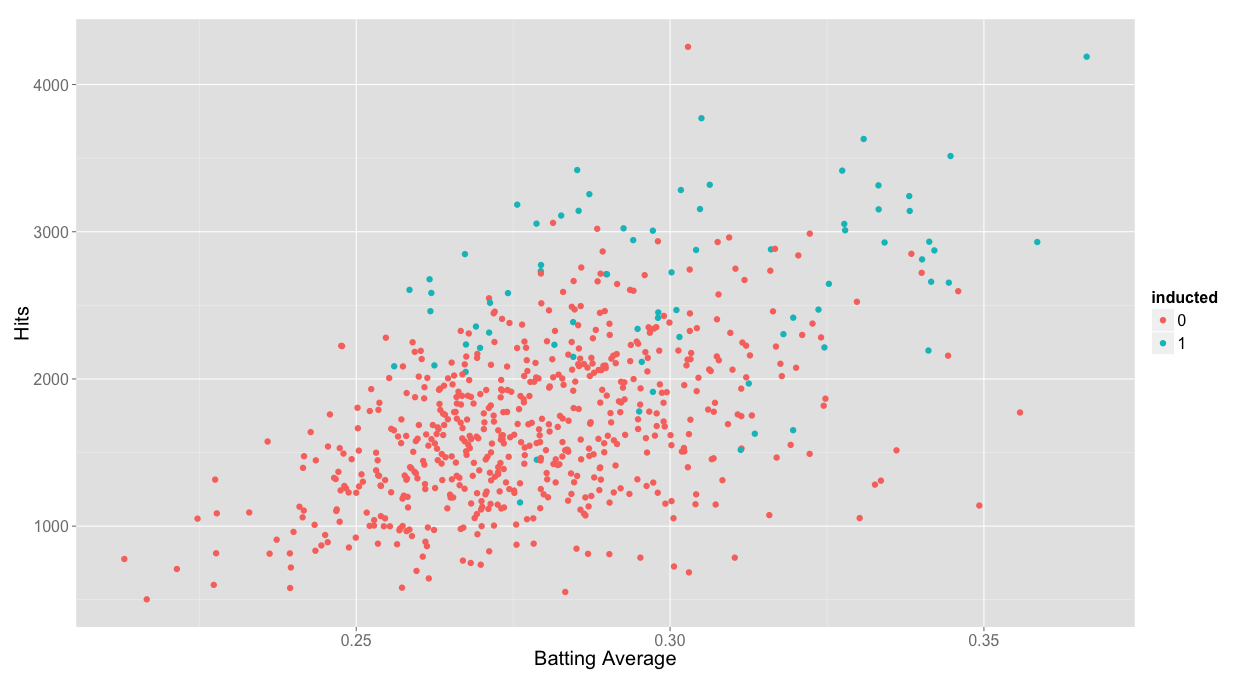
\includegraphics[width=0.9\textwidth]{BAandHits}
	\caption{Batters with more hits and a higher batting average are inducted}
\end{figure}

We can see that more hits and a higher batting average seem to correlate with induction. This makes sense, as one often judges the quality of a batter by his batting average, the numbers of hits a player has per at-bat. The interplay between all of these statistics will be elucidated in more details in the sections to follow. Keep in mind that a lot of the players with many hits and a high batting average that weren't inducted are those players who's induction we seek to predict. Also, That player with over 4000 hits who is not in the Hall of Fames is Pete Rose, who received a lifetime ban from baseball activity for gambling against his own team.


% \begin{figure}[h]
% 	\centering
% 	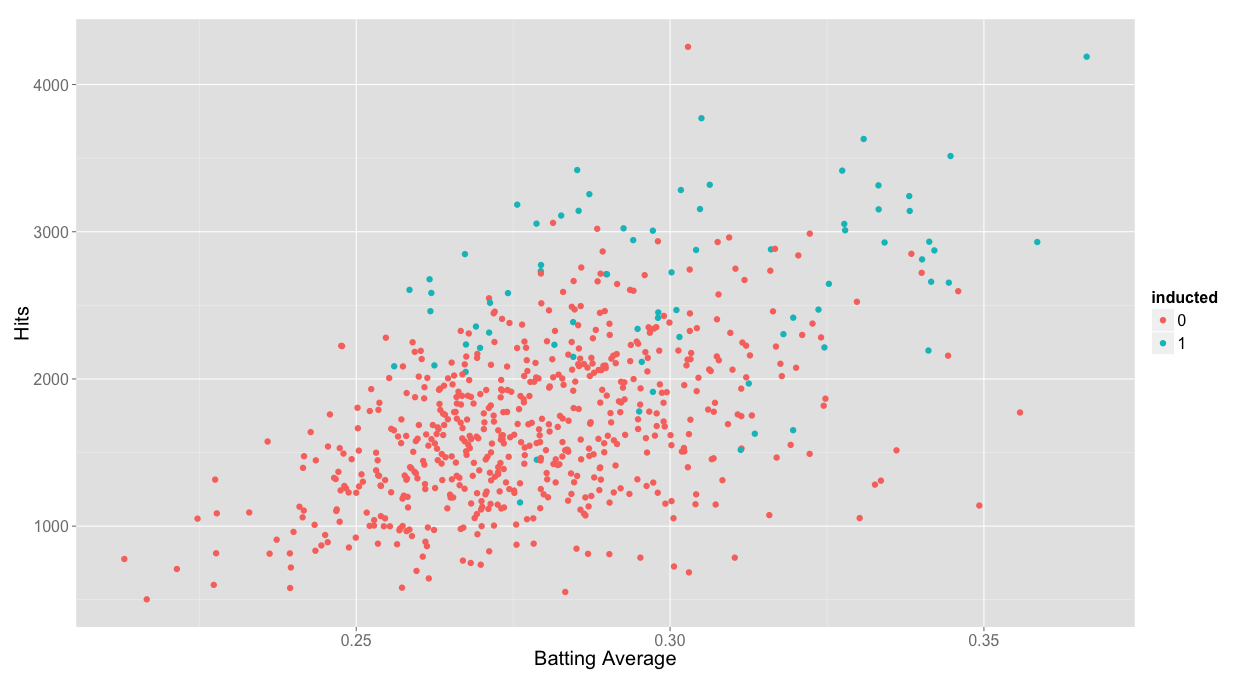
\includegraphics[width=1\textwidth]{BAandHits}
% 	\caption{Batters with more hits and a higher batting average are inducted}
% \end{figure}



% here is where we can add citations
%Maecenas \cite{Smith:2012qr} fermentum \cite{Smith:2013jd} urna ac sapien tincidunt 


\section{Tree-Based Methods for Classification}
\label{method}

In this section, we will give an account of two learning methods that we will use for the basis of prediction: classification trees, and an ensemble method, random forests. We will also introduce the concept of bootstrap aggregating (bagging) which is a fundamental ingredient of random forests. The information here is theoretical, and will be motivated by a simple example. We will encounter applications of these ideas to our HOF data in the next section.
\begin{figure}[h]
	\centering
	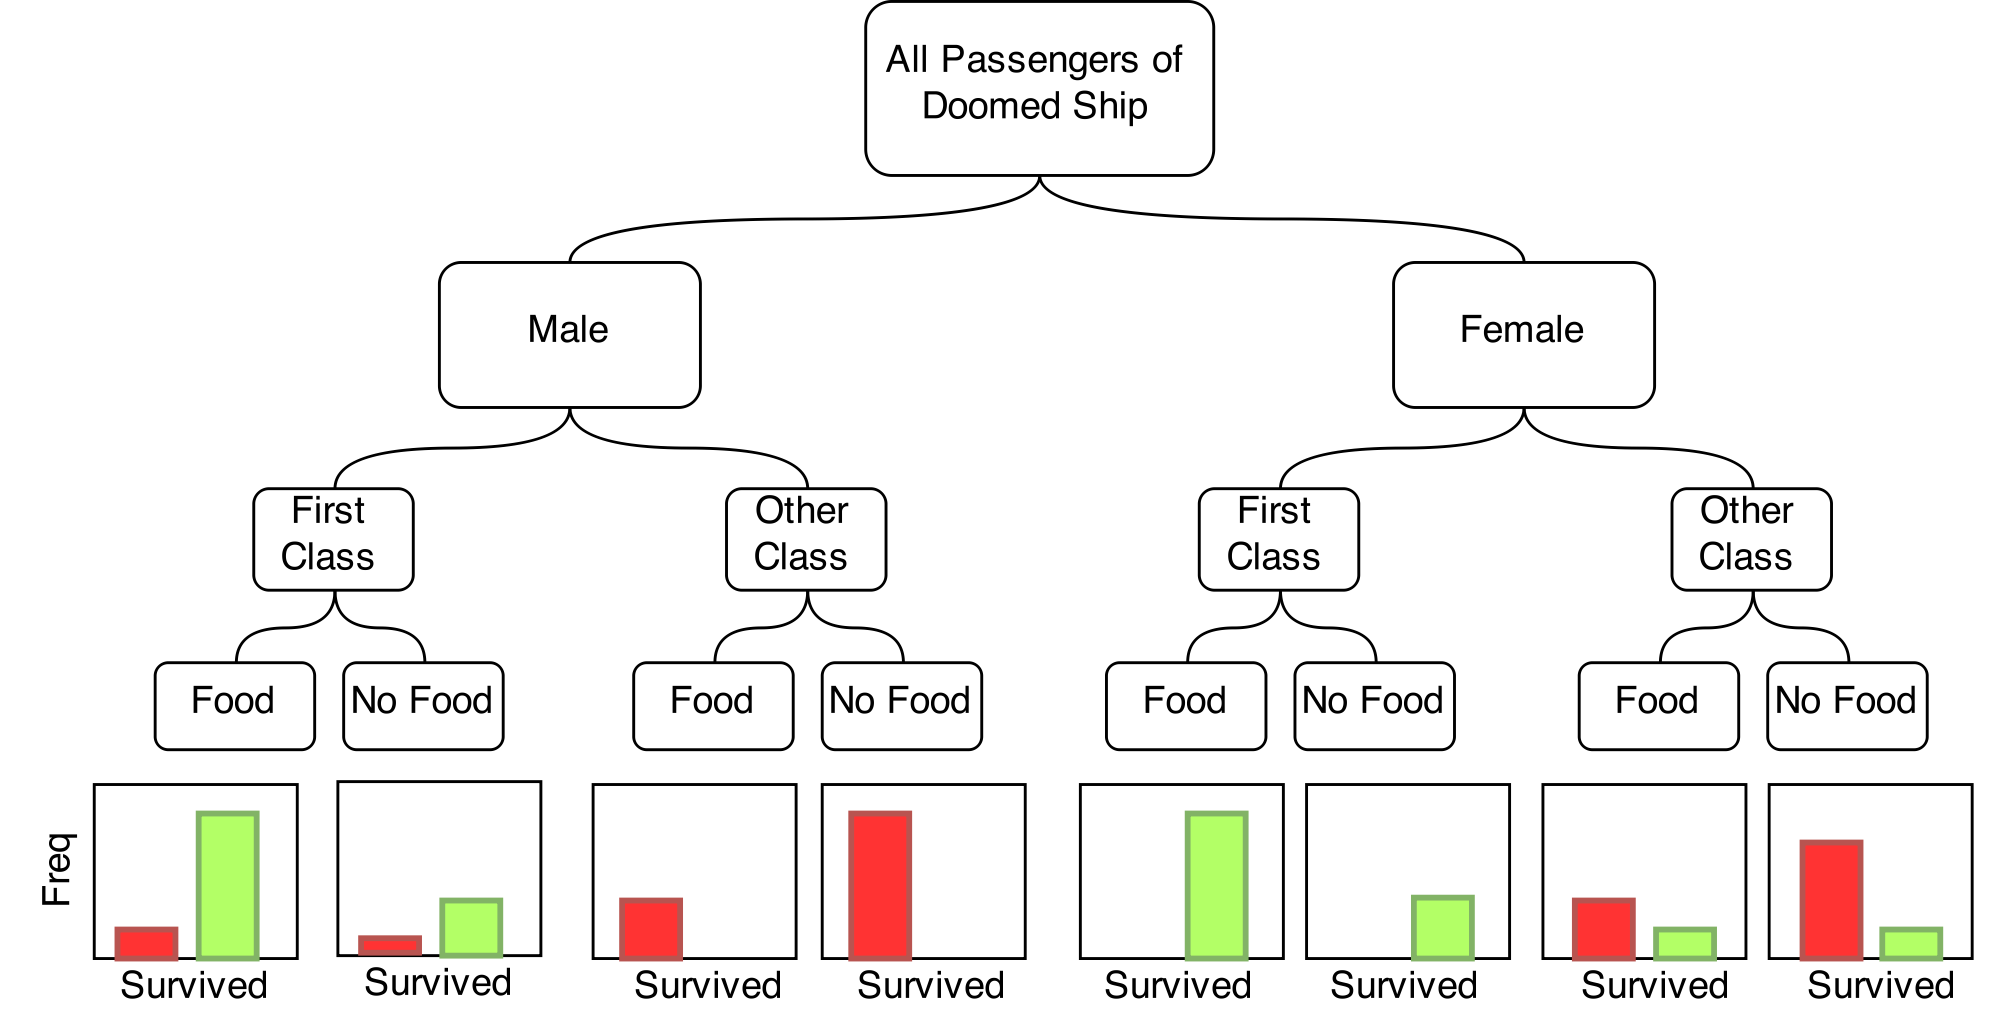
\includegraphics[width=1\textwidth]{TreeExample}
	\caption{Decision Tree for Survival of Boat Disaster}
	\label{fig:SampleTree}
\end{figure}
\subsection{Classification Trees}
Classification trees are a fairly effective predictive tool that are lauded for their high degree of interpretability. When constructing a classification tree, we begin with the full set of observations and begin dividing the predictor space into non-overlapping regions by means of binary splitting. In prediction, we assign each observation in a given region of the predictor space to the most commonly occurring class of the training observations in that region. 

When choosing splits in our tree, we are concerned with the \textit{Gini Coefficient} at each split. We want to choose the feature to split on based on which feature split will give us the greatest decrease in this value. The Gini Coefficient is a measure of how often a randomly chosen element from the set would be incorrectly labeled if it were randomly labeled according to the distribution of labels in the subset. The Gini Coefficient can be computed by summing the probability of each item being chosen times the probability of a mistake in categorizing that item. It reaches its minimum, $0$, when all cases in the node fall into a single target category. This defined as:

$$G = \sum\limits_{i=1}^m p_{i}(1-p_{i}) = 1 - \sum\limits_{i=1}^m p_{i}^{2}$$

\noindent where $i$ takes on values in $\{1,2,\ldots,m\}$, the number of different categorical labels, and $p_i$ is the fraction of items labeled with value $i$ in the node. So $G$ can be seen as a measure of total variance across the $m$ classes. Since this paper will only be discussing a classification variable that takes on 2 values, inducted or not-inducted, in our case $m=2$. Note that $G = 0$ when all observations in that node fall into one class. In splitting at nodes, we look to minimize this value.

Let us illustrate this with a very simple example of a decision tree created to predict the survivors of a boat disaster, show in Figure \ref{fig:SampleTree}. The root node contains all passengers of the ship. We then split the full set of observations according to their sex, followed by a split on what type of ticket they had, followed lastly by a split on whether or not they chose to order a meal with their ticket. Below each terminal node is a distribution of those passengers who survived and those who didn't. 

The tables below show the fates of all passengers based on their ticket type. Now, we can consider the Gini Coefficient associated with the nodes occurring after the split on ticket type from the node labeled ``male'' in the decision tree.

\begin{table}[h]
\begin{tabular}{|l | l l | l|}
\hline
 Male & Survived & Died & total\\
\hline
First & 122 & 19 & 141 \\
Other & 12 & 1113 & 1125 \\
\hline
total & 134 & 1132 & 1286 \\
\hline
\end{tabular}
\quad
\begin{tabular}{|l | l l | l|}
\hline
Female & Survived & Died & total\\
\hline
First & 101 & 2 & 103 \\
Other & 69 & 809 & 878 \\
\hline
total & 170 & 811 & 981 \\
\hline
\end{tabular}

\caption{Aftermath of a Tragic Boat Disaster}
\end{table}

\noindent If we split this subest of the observations on ticket type, we can calculate Gini Coefficient for each of the two successive nodes as follows, with $i=0$ indicating survival and $i=1$ indicating death:

$$G(\textrm{male, first}) = 1 - \sum\limits_{i=0}^1 p_{i}^{2} = 1 - ((122/141)^{2}+(19/141)^{2}) \approx 0.233 $$

$$G(\textrm{male, other}) = 1 - \sum\limits_{i=0}^1 p_{i}^{2} = 1 - ((12/1125)^{2}+(1113/1125)^{2}) \approx 0.021 $$

\noindent This tells us that knowing that a male was holding a ticket other than first class leads us to a very pure node, that is, one in which we have a substantial amount of information to determine the fate of that passenger. The Gini Coefficient is related the related notion of entropy and can be seen as measures of how informative the answer to a ``yes/no'' question is at the split in a tree. Entropy can also be used in determining splits, and can calculated using the following equation, where $p_{i}$ is the same quantity as defined above: 
$$-\sum\limits_{i=0}^m p_{i}log_{2}p_{i}$$

Decision trees, while useful, have their limitations. Firstly, it is possible to grow overly complex trees that overfit the training data \cite{ISLR}. This can happen if we grow our tree in such a way to have only a single observation at each terminal node. The misclassification rate in our training sample would be $0$, but we would be very likely to encounter an error in our training set. In such cases, a method known as pruning is required to combat this problem. \textit{Cost complexity pruning} is a method for considering subtrees of our initial tree model that minimize the cost-complexity criterion, which is defined as follows\cite{ESL}:


Let $T_{0}$ be our unpruned decision tree, and define a subtree $T \subset T_{0}$ to be any tree that can be obtained by collapsing any number of internal (non-terminal) nodes. Let $|T| = |\{R_{1}, R_{2}, \ldots, R_{m}\}|$ denote the number of terminal nodes of our subtree. Define the number of observations at each terminal node as:

$$N_{m} = |\{x_{i} \in R_{m}\}| $$

\noindent And the cost-complexity criterion:

$$C_{\alpha}(T) = \sum\limits_{m=1}^{|T|} N_{m}G_{m}(T) + \alpha|T|$$

For each $\alpha$, there is a unique smallest subtree $T_{\alpha} \subseteq T_{0}$ that minimizes $C_{\alpha}(T)$ An estimation  $\hat{\alpha}$ is done by using tenfold cross-validation, and the final pruned tree is $T_{\hat{\alpha}}$. In tenfold cross validation, the original training set is partitioned into ten equal subsamples, nine of which are used to train are used to train the model, and one used for validation. This process is repeated 10 times, each time selecting a different subsample as the test data. The 10 results from are then averaged to produce a single estimation. More details can be found in Breiman et al.\cite{Breiman1984}

Using our Boat example, we note that that our tree has 8 terminal nodes. If we take a look at the distributions below the nodes, we note that the split on food option is not that meaningful in the case of non-first class males and first class females. So let us consider the subtree $T$ show in Figure \ref{fig:Pruned} formed by removing these splits. We note that the Gini Coefficients of the nodes that precede the removed nodes are already equal to $1$, indicating that we already have perfect information about the survival of these passengers. Splitting these nodes further by food option does not decrease the Gini Coefficient and therefore brings us no new information and can be pruned from our tree. Note that $C_{\alpha}(T) \leq C_{\alpha}(T_{0})$.

\begin{figure}[h]
	\centering
	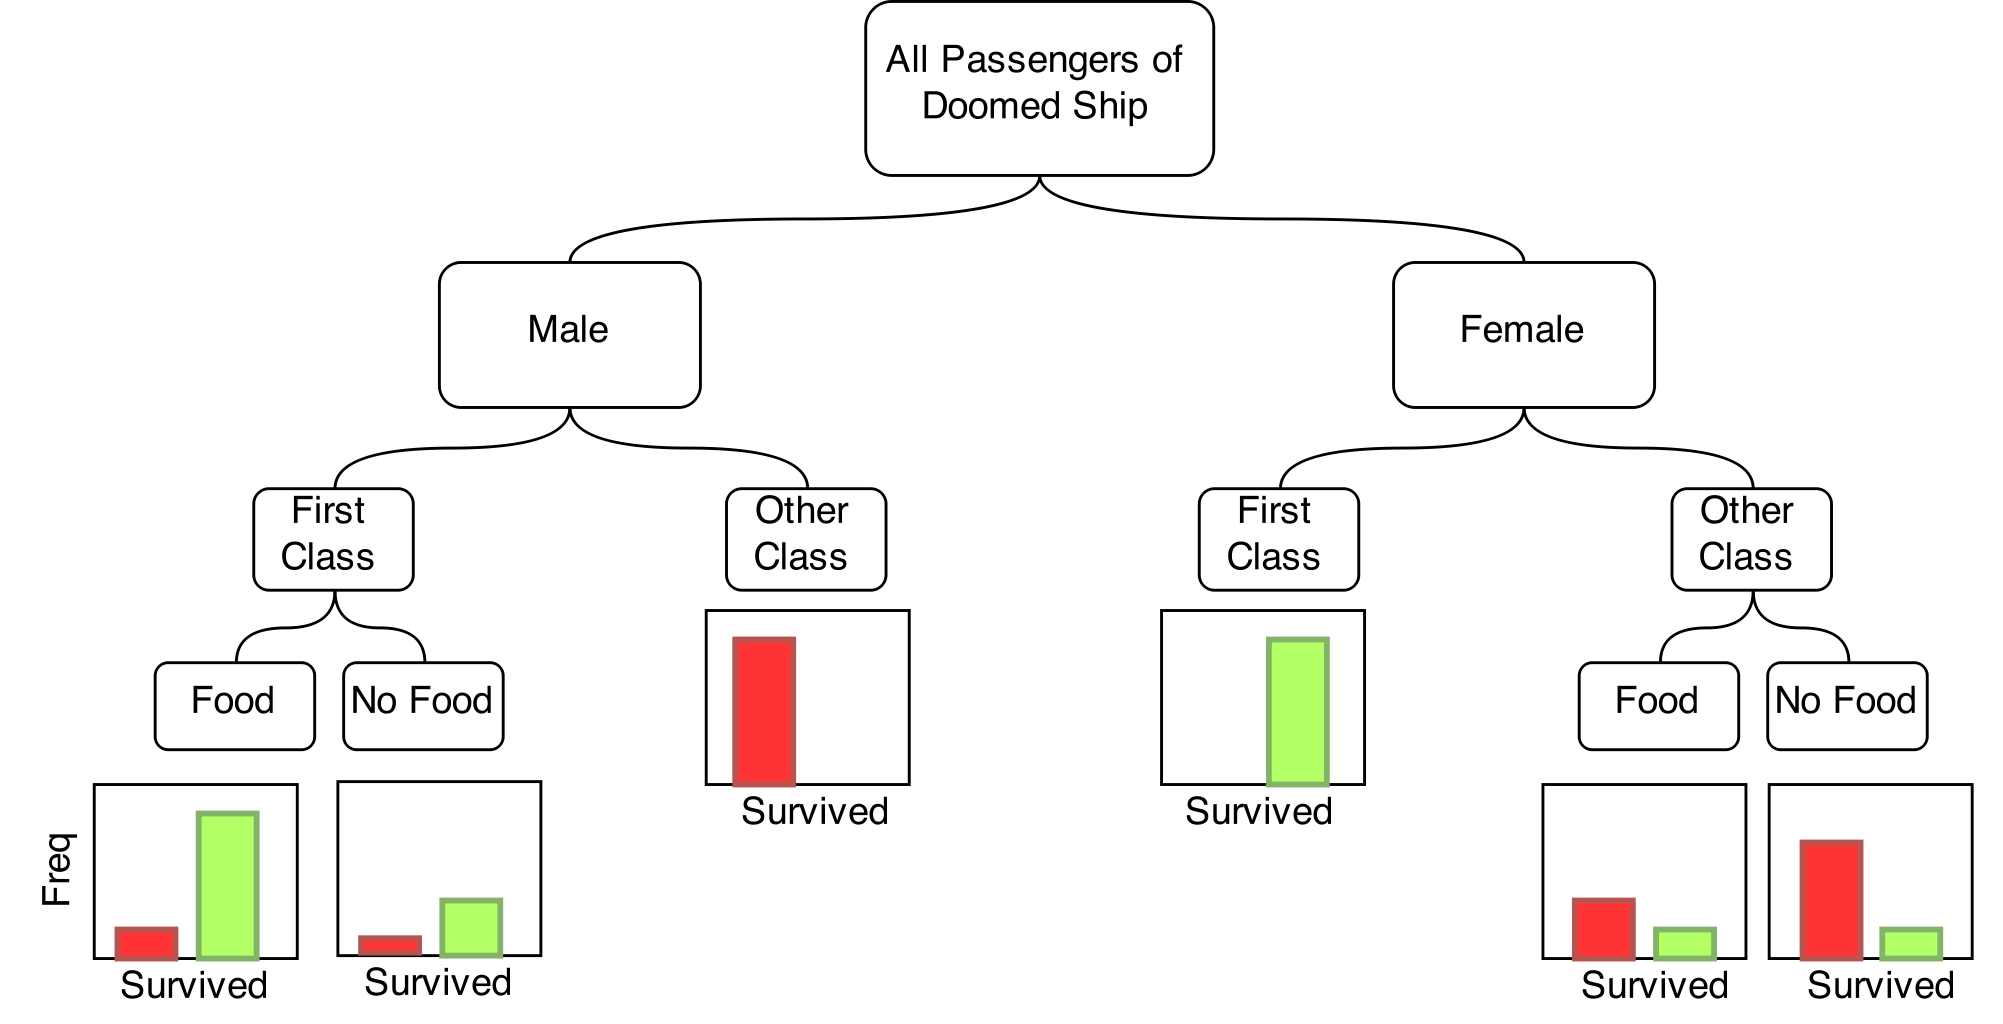
\includegraphics[width=1\textwidth]{PrunedBoat}
	\caption{A less complex version of our tree}
	\label{fig:Pruned}
\end{figure}

\subsection{Ensemble Methods}
Ensemble methods use multiple learning algorithms to obtain better predictive performance than could be obtained from any of the individual learning algorithms composing the ensemble. Here, we look at two such methods, bagging and random forests.


\subsubsection{Tree Bagging}
Decision trees as discussed in the previous section often suffer from high variance in the case of complex trees, meaning that if we fit a decision tree to two random samples from a set of training observations, we could end up with vastly different results\cite{ESL}. \textit{Bagging} (bootstrap aggregating) is a method for reducing the variance of any learning method by taking repeated samples from a single training set and taking, in the case of classification, the most commonly occurring class among the bootstrapped predictions. 

On average, each of the $B$ bootstrapped samples will take about two-thirds of the training observations.  The remaining observations that were not used in fitting a bagged tree are referred to as the \textit{out-of-bag} (OOB) observations, and we can predict the target variable for the \textit{i}th observation using each of the trees in which that observation was OOB. This will yield, on average, $B/3$ predictions from which we can predict the classification for the observation by taking majority vote.\cite{ISLR} Using this method, we can get a single OOB prediction for each of our observations, obtaining an OOB error, which is a valid estimate of the test error for the entirety of our bagged model.

Bagging also gives us insight into which of our predictors were the most important in creating our model by looking at the Gini Coefficient. To do so, we take the sum of the amount that the Gini Coefficient has decreased by splitting on a given predictor and take the average over our $B$ trees.

\subsubsection{Random Forest}


\begin{figure}[h]
	\centering
	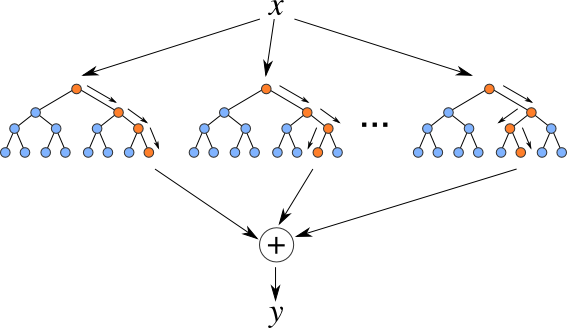
\includegraphics[width=0.6\textwidth]{RF}
	\caption{Random Forest. For classification, a prediction for \textbf{y} is made by majority vote.}
\end{figure}

The random forest technique is quite similar to taking bagged  samples of trees, with the main difference being that at each of the splits only a random sample of size $m < p$ of the set of all predictors $p$ is considered. Typically, $m \approx \sqrt{p}$ predictors suffice\cite{Breiman2001}. This technique helps to decorrelate the tree, as there may be one predictor that has a very high influence in classification. In the case of bagging, this predictor will most likely be used as the first split in a majority of the trees, causing most bagged trees to be quite similar and correlated. By forcing each split to consider on a subset of the predictors, on average $(p-m)/p$ of the splits will not consider this strong predictor\cite{Breiman2001}.


In this paper, we will be utilizing the \textit{randomForest} package in R. 

\section{Prediction Models}

In this section, we apply the techniques introduced in the last section to our HOF data. We will start by creating a single classification trees and then predicting the induction classifier of our training data based on our model. We will also look at some metrics that will allow us to test the effectiveness of our classification model in order to see what parameters would be best to use. 

\subsection{Classification Tree}

\begin{figure}[h]
       \centering 
       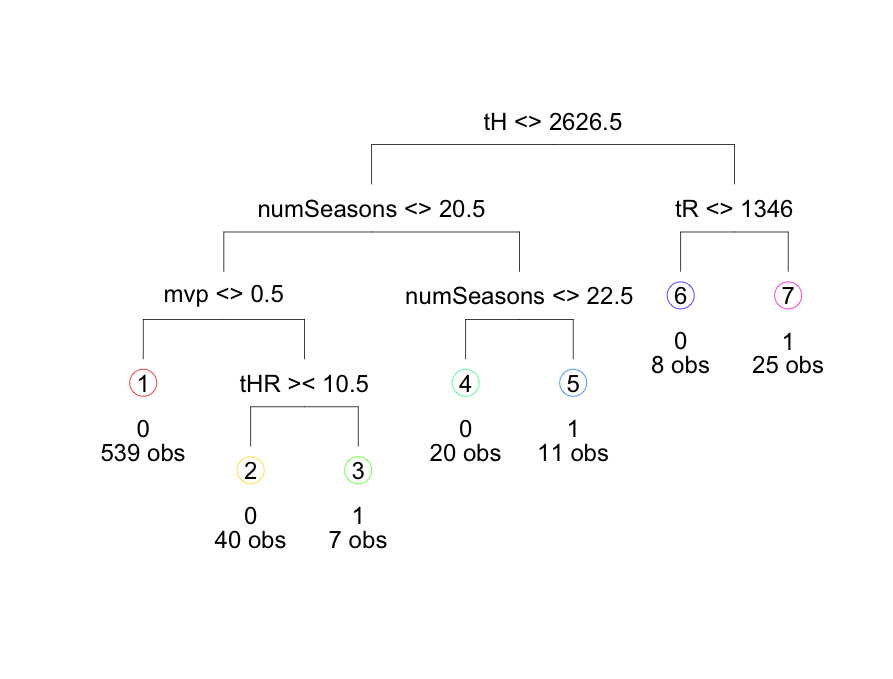
\includegraphics[width=\linewidth]{BatterUnpruned}
       \caption{Batting}
       \label{unprunedBat}
 \end{figure}

 \begin{table}[h]
\centering
\begin{tabular}{|l |l l|}
\hline
 unpruned &  actual & \\
\hline
prediction & 0 & 1 \\
0 & 356 & 23 \\
1 & 23 & 27 \\
\hline
%\caption{Confusion Matrix of test data using pruned tree}
\end{tabular}
\quad
\begin{tabular}{|l |l l|}
\hline
 pruned &  actual & \\
\hline
prediction & 0 & 1 \\
0 & 369 & 35 \\
1 & 10 & 15 \\
\hline
%\caption{Confusion Matrix of Test Data using unpruned tree}
\end{tabular}
\caption{Confusion Matrices for unpruned and pruned decision trees}
\label{conf}
\end{table}

Using R's rpart package, we can fit a classification tree to our data. To do so, we will split the entire data set into a training and a test set and build our tree using the training data. As our training set, we will take a random sample of about $2/3$ of our data. This amounts to $\approx 650$ batters. The tree shown in figure \ref{unprunedBat} was obtained by predicting induction based on all of our features mentioned in section \ref{data}. Our model produced a tree with eight splits and 9 terminal nodes and we notice that only 5 variables were used in the creation of the tree: tH, numSeasons, tR, mvp, tHR. The misclassification error of this tree on the training data was : $62/650 \approx 9.5\%$. Let's use this model on our test data to see how it performs.




\begin{figure}[h]
       \centering 
       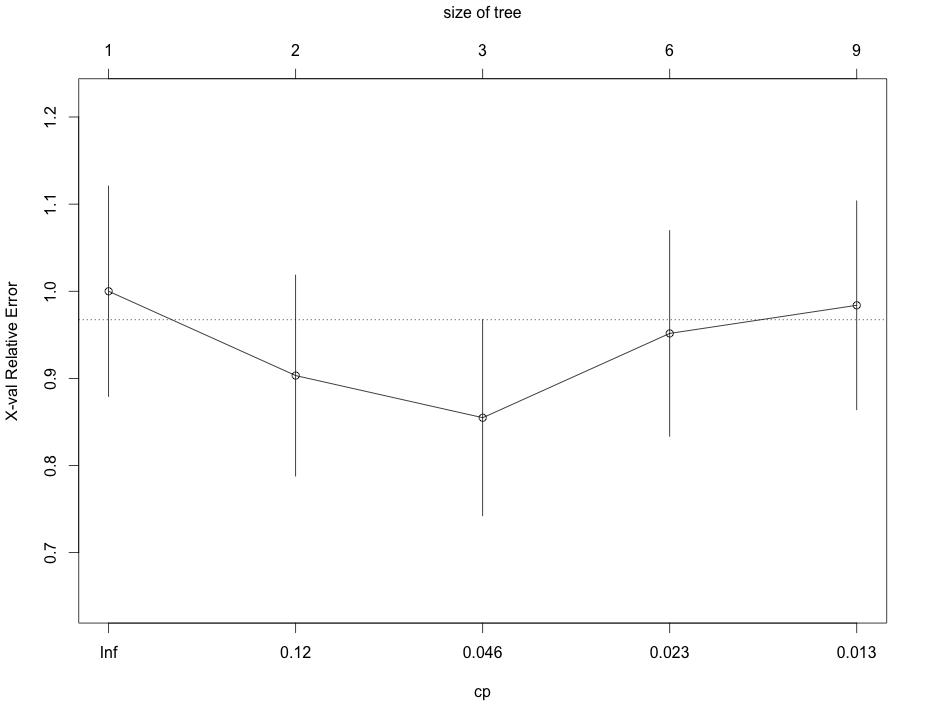
\includegraphics[width=0.85\textwidth]{PlotCP}
       \caption{Complexity Parameter of Various Trees}
       \label{CPlot}
 \end{figure}


\begin{figure}[h]
       \centering 
       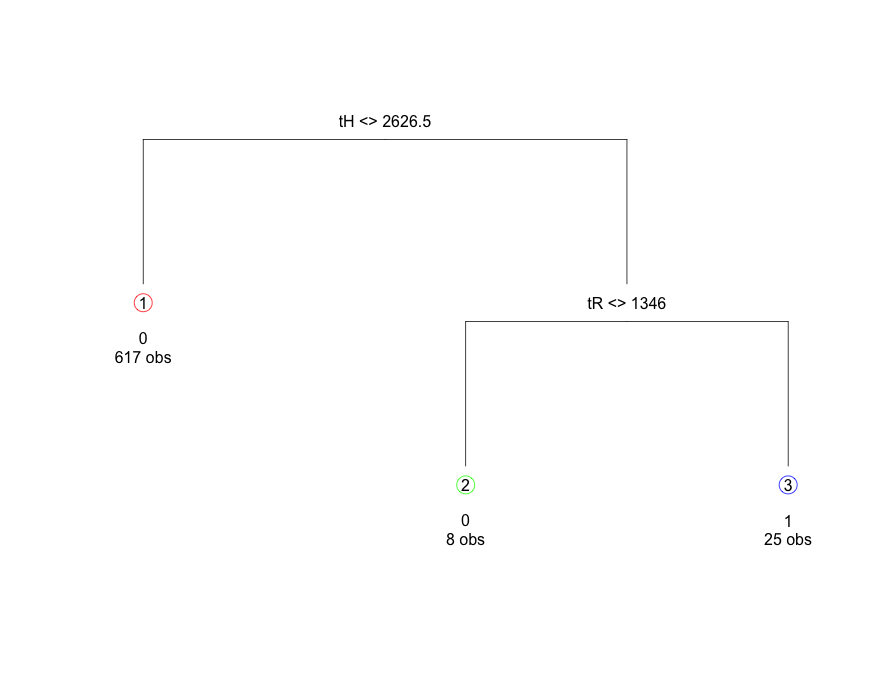
\includegraphics[width=0.75\linewidth]{BattersPruned}
       \caption{Our Pruned Tree}
       \label{pruned}
 \end{figure}

Our model predicted the induction of our test players with a misclassification rate of $1 - 383/429 \approx 10.7\%$. We can perform cross validation on the tree to see if there is a more ideal pruned tree size. Having a look at figure \ref{CPlot}, we notice that the cross validation error is minimized around cost complexity parameter (cp) $0.046$. We can use this value to prune our original tree in hopes of obtaining a more stable model of size 3. Generating a new tree model having only 3 terminal nodes actual performs slightly better than our original tree, with a misclassification rate of $1-384/429 \approx 10.4\%$ on the test data. This data is summarized in table \ref{conf}.





% Now, to test the performance of this tree, we must estimate a test error by predicting a player's hall of fame induction on our test data. We will look at how our classification model performed.

% \begin{lstlisting}
% tree.pred=predict(tree.hof,HallOfFame[-train,],type="class")
% with(HallOfFame[-train,],table(tree.pred,inducted))
%          inducted
% tree.pred   0   1
%         0 203  11
%         1  19  18
% \end{lstlisting}

% This tells us that we have a misclassification rate of $1-(203+18)/(203+18+11+19) \approx 12\%$. We will see if this can be improved by using the tree package's pruning feature. The goal of pruning a decision tree is to reduce the complexity of our model, and to reduce overfitting. A pruned tree is simply a less complex tree chosen from set of all subtrees of our decision tree. The method used by the tree package in R is \textit{cost complexity pruning}, which operates as follows: Rather than considering every subtree of our initial tree, we only consider a sequence of trees that is indexed by a tuning parameter $\alpha$. The goal of pruning is to select a subtree that will lead to the lowest misclassification error rate. Such an $\alpha$ can be chosen by using cross-validation on our initial tree.\textbf{talk about cv and pruning more?}


\subsection{Random Forest}
In this section, we will build a model for predicting hall of fame induction using an ensemble of decision trees. The method is similar to the one followed above, except in this case we will use bagging to ensure that we do not overfit the training data. Instead of building just a single tree in which all variables are considered at each binary split, we will build numerous decision trees in which a randomly selected variable is chosen at each split. As before, each tree is trained using a training set, and the trees are built so that each terminal node is \textit{pure} in the sense that all of the observations in the node fall into the same class.

The test data will be referred to as \textit{out-of-bag} sample, since it is not included in bagging method used for training. The prediction for the out-of-bag samples will be the majority vote of the predictions from the individual trees. To change things up, in this section we will be considering the full set of batters rather than simply those that have appeared on at least one ballot. This will be useful in predicting induction for players that have not yet retired, or have retired in the last 5 years.

To do this, we will make our training set all players that have retired before 2009 and our test set all players who are still currently active, or have retired after 2009. We will arbitrarily choose to grow a forest of 1000 trees, and use a tuning function to determine how small of a subset of our variables should be chose from at each split. Figure \ref{mtry} indicates that 3 variables will suffice and result in the lowest OOB-error for 1000 trees. This low OOB-error for choosing 3 variables at each split indicates that OOB observations were misclassified most infrequently in such a scenario.

\begin{figure}[h]
       \centering 
       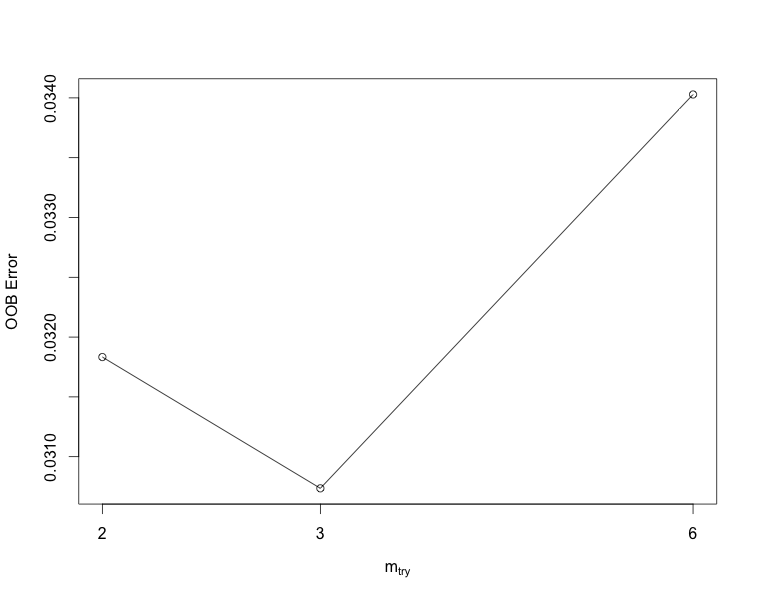
\includegraphics[width=0.85\linewidth]{mtry}
       \caption{number of variables again OOB-error}
       \label{mtry}
 \end{figure}

After training our forest, the results in table \ref{rfconf} were obtained, indicating an OOB-error rate of $\approx 2.96\%$ We see that the misclassification rate for non HOF players is much lower than that of players who were inducted. This is due to the fact that there is a much larger population of non HOF players, making them easier to classify by the model. 

A benefit of random forests is that they can indicate which variables were most important in prediction. This is a measure of the total amount that the Gini Coefficient is decreased by splits over a given variable and then averaged over all the trees in the forest. In our case, the results in table \ref{varImp} show that All Star Game appearances followed by the total number of runs, rbis, and hits are the factors that best classify a HOF batter.

\begin{table}[h]
\centering
\begin{tabular}{|l |l l|}
\hline
 rf &  actual & \\
\hline
prediction & 0 & 1 \\
0 & 851 & 10 \\
1 & 17 & 3 \\
\hline
\end{tabular}
\caption{Confusion Matrix of training data in random forest model}
\label{rfconf}
\end{table}

\begin{table}[h]
\centering
\begin{tabular}{|l |l|}
\hline
 variable & MeanDecreaseGini\\
\hline
ASgame & 25.511962 \\
tR     & 18.343892 \\
tRBI   & 12.891316 \\
tH     & 12.077022 \\
tHR    &  7.500770 \\
mvp    &  5.923212 \\
tBA    &  5.071497 \\
tSB    &  4.261315 \\
gg     &  2.661624 \\
\hline
\end{tabular}
\caption{Variable Importance}
\label{varImp}
\end{table}

Now we are in a position to use our random forest model to predict hall of fame induction on the test set, shown in table \ref{rfplayers}. Since our test set contained player not yet eligible for induction, these prediction can best tested against actual data once these players appear on ballots. It should be noted that these predictions were made as if all of the players in our test set had retired \textit{today}. Since nothing in our model projects players' performance in the future, there are definitely some players that are worthy, but just haven't had enough playing time to accumulate the required statistics. For example, in table \ref{rfplayers}, we see that Miguel Cabrera is not HOF worthy. However it is incredibly impressive that he still has around 10 years left in him and he is already fairly close to being at a point where his career statistics get him into the hall.


\begin{table}[h]
\centering
\begin{tabular}{|l |l |l|}
\hline
player & inducted & percent of ballots\\
\hline
Rodriguez, Ivan & 1 & 0.842 \\
Sheffield, Gary & 1 & 0.810 \\
Ramirez, Manny & 1 & 0.800 \\
Pujols, Albert & 1 & 0.798 \\ 
Griffey, Ken & 1 & 0.781 \\
Guerrero, Vladimir & 1 & 0.733 \\
Suzuki, Ichiro & 1 & 0.728 \\
Jeter, Derek & 1 & 0.558 \\
Rodriguez, Alex & 1 & 0.553 \\
Jones, Chipper & 1 & 0.517 \\
Mauer, Joe & 0 & 0.421 \\
Thome, Jim & 0 & 0.410 \\
Delgado, Carlos & 0 & 0.373 \\
Cabrera, Miguel & 0 & 0.368 \\
Ortiz, David & 0 & 0.336 \\
\hline
\end{tabular}
\caption{A few predictions from our random forest}
\label{rfplayers}
\end{table}


 


\section{Conclusion}
Decision trees and random forests are just 2 learning methods that can be used for classification or regression. There are numerous other models including linear regression, support vector machines, nearest neighbors, neural networks, and logistic regression, just to name a few. The methods chosen here were done so to illustrate their effectiveness and interpretability.

As we have seen, decision trees can suffer from overfitting the training data, and appear to perform worse in comparison to random forests. Decision trees are advantageous since they appear to mimic the human decision making process for classifying observations as seen with our description of the Gini Coefficient. They can also be neatly depicted in a graph, aiding in presentation. Also, as we have seen, the downsides of decision tree learning can be remedied by aggregating them in a random forest.

With regards to the Hall of Fame Data, we have shown that our decision tree model was able to predict induction with about 90\% accuracy. The difference between an urpuned and a pruned model was quite minimal with respect to accuracy, but quite substantial for interpretability. We can think of the outcome of the unpruned tree in the following way:


\begin{enumerate}
	\item Did the player have at least 2327 hits in his career?
	\item If yes, did the player score more than 1346 runs?
	\item If yes, this player will be inducted with 90\% certainty. 
\end{enumerate}

Random forests performed much better in prediction, with a misclassification error rate near 3\%. The model we created with the random forest technique was also more informative, as we took advantage of the power of the method and used the full set of batters. We were also able to view the important of each variable in deciding whether or not a player would be inducted. This can prove to be useful evaluating the patterns of voters and indicating periods of time where they too heavily favor one statistic. For example, all star game selection is done by the general public, and players from higher market teams often make the all star team not because of their talent, but because of the higher population of voters in their region.

Going along with this, some interesting extensions of this model could be formed by doing time series analysis on voting patterns. This could indicate certain eras in which BBWAA voters were more interested in one statistic over another, and classifying the types of batters most lauded during that era. For example, in the early 2000s during the height of steroid use power hitters were held in higher regard than ``scrappy'' players, while now we are in an offensive lull, where high contact batters are more vital to a teams' winning a game.

%% References
%%
%% Following citation commands can be used in the body text:
%% Usage of \cite is as follows:
%%   \cite{key}          ==>>  [#]
%%   \cite[chap. 2]{key} ==>>  [#, chap. 2]
%%   \citet{key}         ==>>  Author [#]

%% References with bibTeX database:
\section{References}
\bibliographystyle{model1-num-names}
\bibliography{sample.bib}

%% Authors are advised to submit their bibtex database files. They are
%% requested to list a bibtex style file in the manuscript if they do
%% not want to use model1-num-names.bst.

%% References without bibTeX database:

% \begin{thebibliography}{00}

%% \bibitem must have the following form:
%%   \bibitem{key}...
%%

% \bibitem{}

% \end{thebibliography}


\end{document}

%%
%% End of file `elsarticle-template-1-num.tex'.